\section*{Contexte Physique}
\addcontentsline{toc}{chapter}{Environnement spatial : le Soleil, ses événements et leurs effets sur la Terre}

\section*{Physique Solaire}
\addcontentsline{toc}{section}{Physique solaire}



\begin{wrapfigure}[19]{r}{0.5\linewidth}
\centering
   \includegraphics[width=\linewidth]{images/Sun layers.png}
    \caption{\centering Representation of the Sun layers (not to scale); \\ Source: Reames 2021} %\cite{reames_solar_2021}}
    \label{fig:layers}
\end{wrapfigure}

Notre Soleil est une étoile moyenne, quand il s’agit de sa taille et de sa masse. 
Le Soleil est à peu près au milieu de sa vie, dans sa longue « stabilité »\footnote{Cette stabilité est relative, comme nous le verrons dans les sections suivantes.} période. \\

Le noyau du Soleil fusionne l’hydrogène en hélium, libérant de l’énergie qui se déplace à travers la zone radiative. 
Lorsque cette énergie se déplace à travers les couches extérieures plus froides, des courants convectifs se forment, provoquant la génération de champs magnétiques par le plasma en mouvement.  
Au-dessus de cette zone de convection se trouve la photosphère, la « surface » visible, même si la masse solaire s’étend dans la chromosphère et la couronne, qui constituent l’atmosphère extérieure du Soleil. 
Les couches du Soleil peuvent être illustrées comme dans la Figure \ref{fig:layers}. 


\vspace{5mm}

Le Soleil tourne autour de son axe en environ un mois. Comme notre Soleil n’est pas un corps rigide, sa vitesse de rotation varie de 26 jours à l’équateur à 33 jours à 75 degrés. 
Ce phénomène est appelé rotation différentielle, et est principalement responsable de toutes les conséquences décrites ci-dessous. 



Le cisaillement entre les différentes couches, causé par la rotation différentielle, perturbe le champ magnétique de l’étoile. 
Le magnétisme solaire est chaotique et instable, et les lignes de champ peuvent former des boucles à l’extérieur de la surface. 
L’intersection des lignes de champ magnétique avec la photosphère provoque l’apparition d’une tache solaire (voir Figure \ref{fig:Sunspots}). 
Ce sont des zones plus sombres et plus froides de la surface car le transport d’énergie convective est supprimé. 
Les groupes de taches solaires forment un \acrlong{ar} (\acrshort{ar}). 


\begin{figure}[h!]
    \centering
    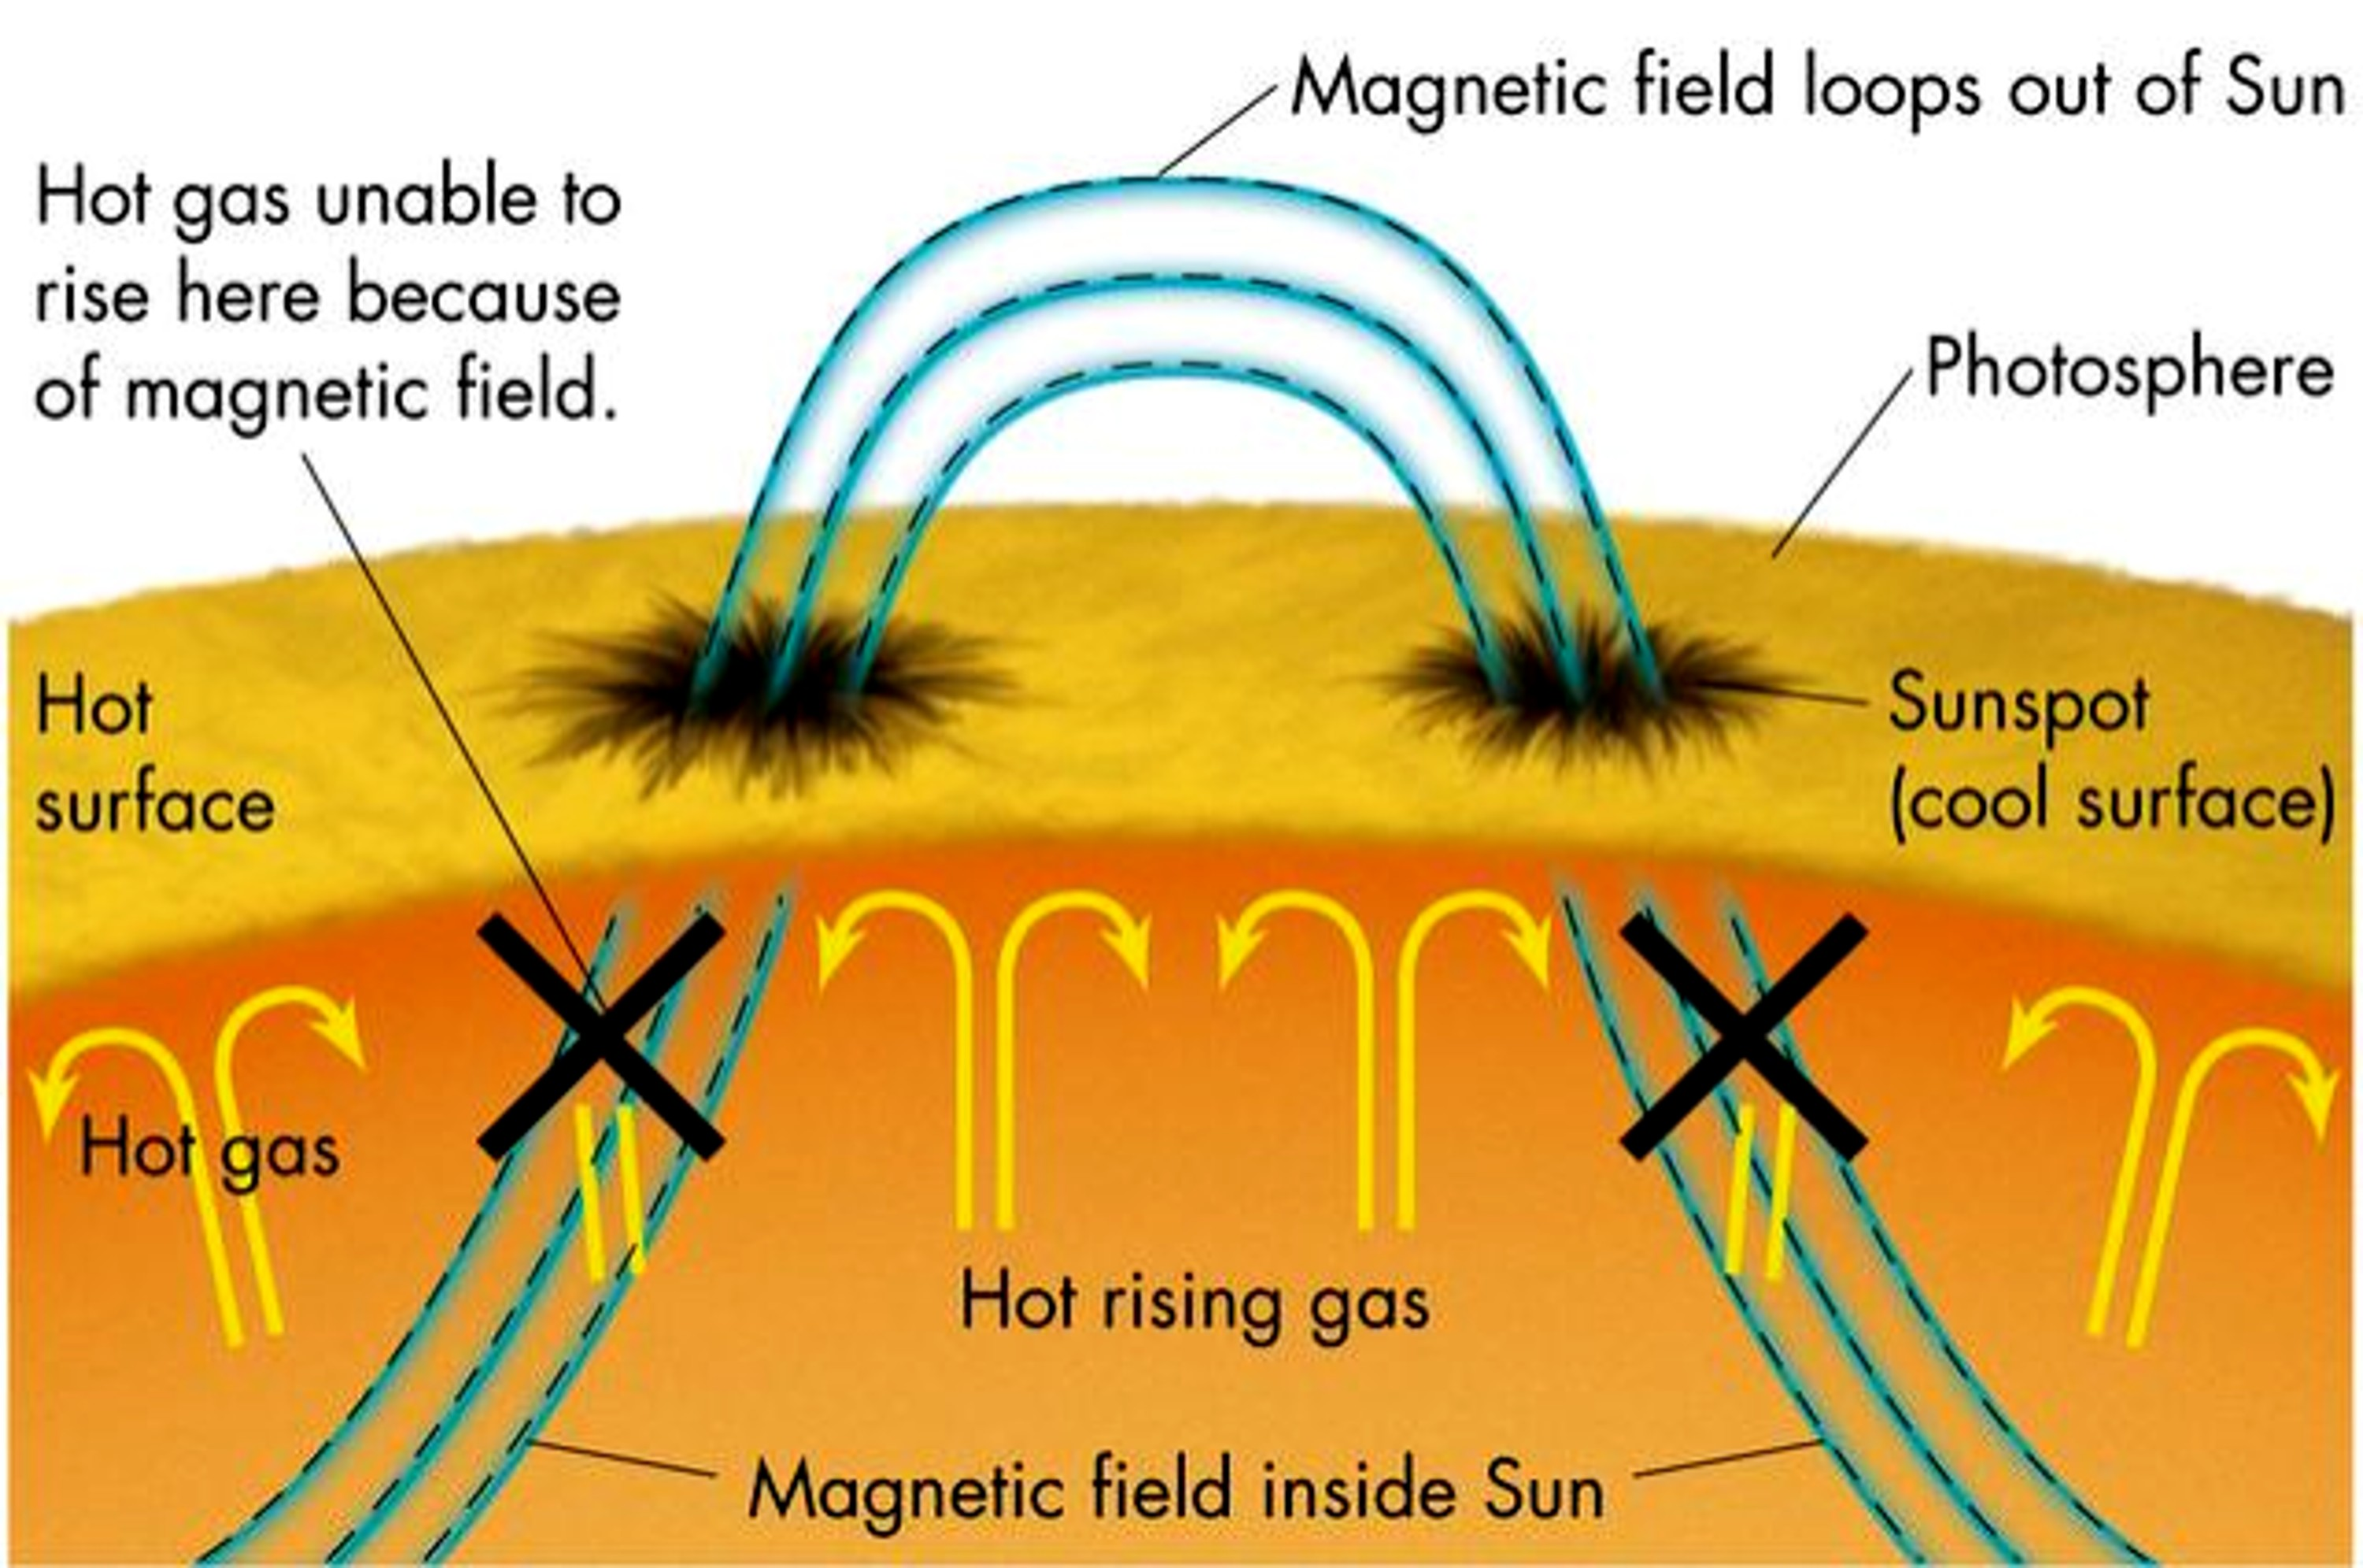
\includegraphics[width=0.8\linewidth]{images/sunspot.jpg}
    \caption{\centering Visualisation de la relation entre les taches solaires et le champ magnétique ; \\Source : \href{https://www.sliderbase.com/prdownload-1152.html}{slidebase.com} (auteur inconnu)}
    \label{fig:Sunspots}
\end{figure}



\section*{Évènements solaires}
\addcontentsline{toc}{section}{Évènements solaires}


Tout ce cisaillement, combiné à une température élevée et un magnétisme chaotique, conduit à des événements puissants tels que les éruptions et les éjections de masse coronale, qui peuvent conduire à des événements \acrshort{sep}. 


\subsubsection{Flare}
Une éruption solaire est une émission relativement rapide, intense et localisée de rayonnement électromagnétique provenant d’un \acrshort{ar}. 
Nous pouvons facilement observer ce phénomène en observant différentes longueurs d’onde telles que l’EUV ($\approx 10-100~\text{nm}$) ou les rayons X ($\approx 10^{-3}-10~ \text{nm}$). 
Une grande éruption visible est représentée sur la figure \ref{fig:flare}. 


\subsubsection{Coronal Mass Ejection}

Les éjections de masse coronale ("\acrlong{cme}s"; \acrshort{cme}s) sont de grandes expulsions de plasma et de champ magnétique provenant de la couronne solaire. 
Elles peuvent éjecter des milliards de tonnes de matière coronale. Une CME se déplace vers l’extérieur du Soleil à des vitesses élevées atteignant parfois 3000 km/s. 
Une CME associée à une grande éruption est représentée dans la Figure \ref{fig:cme}. 

\begin{figure}[h!]
    \centering
    \begin{subfigure}{0.5\textwidth}
        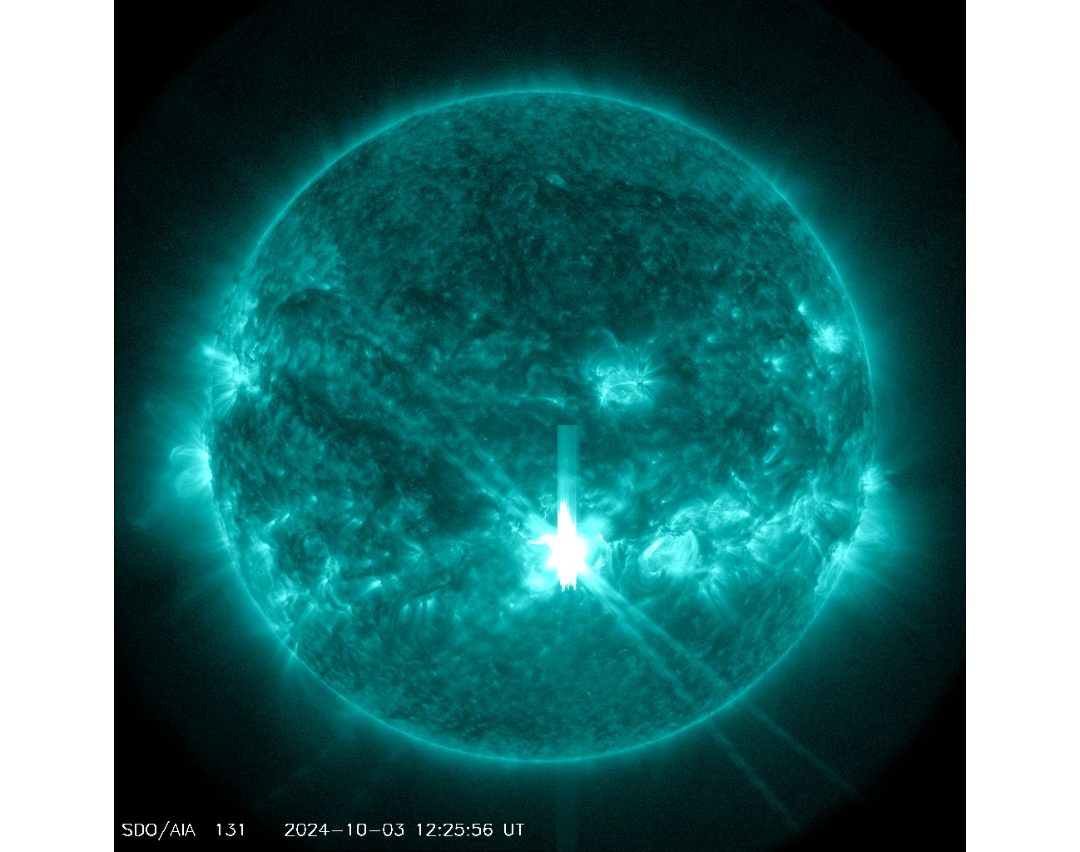
\includegraphics[width=\linewidth]{images/X9 flare.png}
        \caption{\centering Éruption solaire de magnitude extrême (X9.0), capturée par SDO le 3 octobre 2024 ; \\ Source: \href{https://sdo.gsfc.nasa.gov/data/aiahmi/browse/movie.php}{SDO NASA}.}
        \label{fig:flare}
    \end{subfigure}
    \hfill
    \begin{subfigure}{0.4\textwidth}
        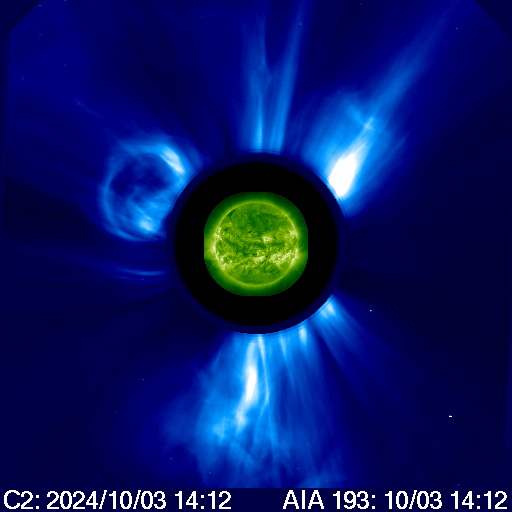
\includegraphics[width=\linewidth]{images/cme.png}
        \caption{\centering CME associé au flare gauche capturée par le coronographe LASCO C2 ; \\ Source: \href{https://cdaw.gsfc.nasa.gov/movie/make_javamovie.php?date=20241003&img1=lasc2aia193}{CDAW NASA}.}
        \label{fig:cme}
    \end{subfigure}
\end{figure}


\subsubsection{Solar Energetic Particles}\label{sep_physic_context}


Un événement \acrshort{sep} est défini comme l’arrivée (généralement sur Terre) d’électrons, de protons et d’autres particules de haute énergie (de une à plusieurs centaines de MeV). 
Dans la littérature, on peut trouver différents seuils qui distinguent un événement du bruit de fond. 
La définition couramment utilisée est celle de la NOAA, qui place le seuil à 10 pfu (1 pfu = 1 proton cm$^{-2}$ s$^{-1}$ sr$^{-1}$) dans le canal des protons $\geq$10 MeV. 
Le canal à protons est généralement pris en raison de ses impacts plus importants sur les astronautes et les satellites.  \\ 

Pour atteindre ces niveaux d’énergie, les particules doivent être accélérées vers des vitesses relativistes. 
Cela peut se produire à la suite de l’occurrence d’un ou d’une combinaison des événements solaires précédemment décrits. 
En effet, nous pouvons expliquer cette accélération par deux phénomènes : 
\begin{itemize}
    \item Le premier phénomène est dû à la reconnexion magnétique des lignes de champ ouvert dans la couronne solaire, donc lié à l’apparition d’une éruption.
    \item La seconde est liée aux ondes de choc chassées du Soleil par une CME. 
\end{itemize} 


\begin{figure}[h!]
    \centering
    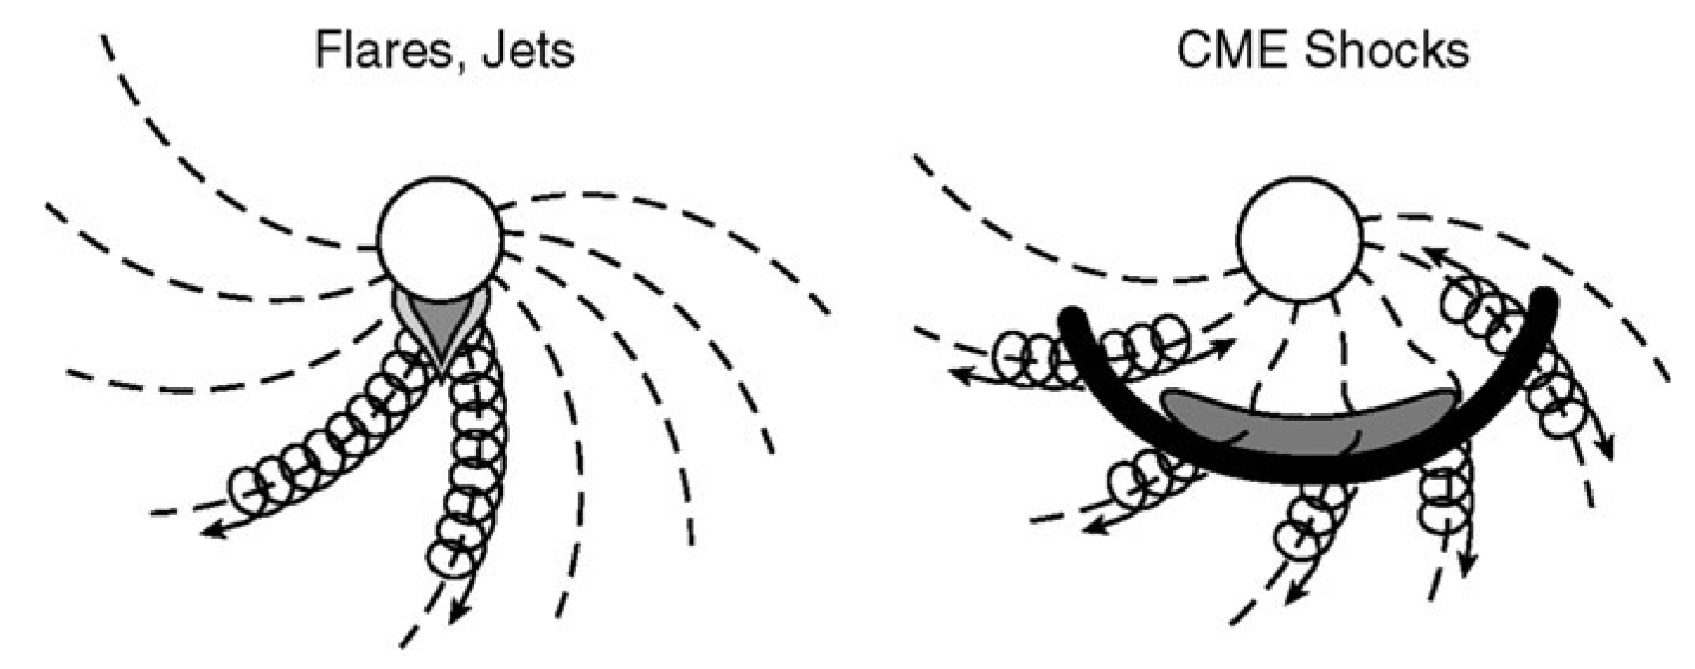
\includegraphics[width=0.65\linewidth]{images/sep events.png}
    \caption{\centering Représentation des deux principaux types d’accélération de particules et leur propagation selon la spirale de Parker ; \\ Source: Reames 2021.}
\end{figure}


\section*{Interactions Soleil-Terre}
\addcontentsline{toc}{section}{Interactions Soleil-Terre}

plutôt l'aspect physique

\section*{Space Weather}
\addcontentsline{toc}{section}{Space Weather}

plutôt l'aspect conséquences sur nos usages quotidien (satellites, aviation, lignes haute tension)